\ifdefined\beamerclass
\else
  \def\beamerclass{beamer}
\fi

\ifdefined\articlemode
  \documentclass[]{article}
  \usepackage[a4paper,margin=2cm]{geometry}
  \usepackage[envcountsect]{beamerarticle}
  \usepackage{parskip}
  \usepackage[hidelinks]{hyperref}
\else
   \documentclass[\beamerclass,ignorenonframetext]{beamer}
\fi


\usepackage{pgfpages}
\mode<handout>{
  % \setbeamercolor{background canvas}{bg=black!20}
  \pgfpagesuselayout{2 on 1}[a4paper,border shrink=5mm]
}

\usepackage{lmodern}
\usepackage{listings}
\usepackage{amsmath}
\usepackage{bm}
\usepackage{textpos} % package for the positioning

\usepackage{pgf, tikz}
\usetikzlibrary{arrows, automata}

\usetheme{Copenhagen}
\hypersetup{pdfstartview={Fit}}
\lstset{basicstyle=\small\ttfamily,breaklines=true}

\usepackage[english]{babel}
\usepackage{algorithm}
\usepackage[noend]{algpseudocode}
\usepackage[utf8x]{inputenc}
\usepackage{graphicx}
\usepackage{hyperref}
%\graphicspath{{./images/}}
\usepackage{tikz}
\usetikzlibrary{shapes.geometric, arrows,chains}
\usepackage{booktabs,makecell,multirow,tabularx}
\usepackage{verbatim}
\renewcommand{\arraystretch}{1.2}
\renewcommand\theadfont{\normalfont\bfseries}
\usepackage{array}
\usepackage{listings}
\lstset{language=Java, showstringspaces=false}
\usepackage[normalem]{ulem}
\usepackage{bm}
\def\layersep{2.5cm}

\usepackage{xcolor}
%\usepackage{subfig}
\setbeamertemplate{caption}{\insertcaption}
\usepackage[caption=false]{subfig}
\usepackage{hyperref}
\usepackage{verbatim}
%\setbeamertemplate{caption}[numbered]%\numberwithin{figure}{section}
% Define block styles
\tikzstyle{decision} = [diamond, draw, fill=blue!20, 
    text width=4.5em, text badly centered, node distance=3cm, inner sep=0pt]
\tikzstyle{block} = [rectangle, draw, fill=blue!20, 
    text width=3em, text centered, rounded corners, minimum height=3em]
\tikzstyle{line} = [draw, -latex']
\tikzstyle{cloud} = [draw, ellipse, fill=red!20, node distance=3cm,
    minimum height=2em]
\tikzset{
  startstop/.style={
    rectangle, 
    rounded corners,
    minimum width=3cm, 
    minimum height=1cm,
    align=center, 
    draw=black, 
    fill=red!30
    },
  process/.style={
    rectangle, 
    minimum width=3cm, 
    minimum height=1cm, 
    align=center, 
    draw=black, 
    fill=blue!30
    },
  decision/.style={
    rectangle, 
    minimum width=3cm, 
    minimum height=1cm, align=center, 
    draw=black, 
    fill=green!30
    },
  arrow/.style={thick,->,>=stealth},
  dec/.style={
    ellipse, 
    align=center, 
    draw=black, 
    fill=green!30
    },
}
\tikzstyle{arrow} = [thick,->,>=stealth]

\tikzset{onslide/.code args={<#1>#2}{%
  \only<#1>{\pgfkeysalso{#2}} % \pgfkeysalso doesn't change the path
}}

\makeatletter
\newenvironment<>{btHighlight}[1][]
{\begin{onlyenv}#2\begingroup\tikzset{bt@Highlight@par/.style={#1}}\begin{lrbox}{\@tempboxa}}
{\end{lrbox}\bt@HL@box[bt@Highlight@par]{\@tempboxa}\endgroup\end{onlyenv}}

\newcommand<>\btHL[1][]{%
  \only#2{\begin{btHighlight}[#1]\bgroup\aftergroup\bt@HL@endenv}%
}
\def\bt@HL@endenv{%
  \end{btHighlight}%   
  \egroup
}
\newcommand{\bt@HL@box}[2][]{%
  \tikz[#1]{%
    \pgfpathrectangle{\pgfpoint{1pt}{0pt}}{\pgfpoint{\wd #2}{\ht #2}}%
    \pgfusepath{use as bounding box}%
    \node[anchor=base west, fill=orange!30,outer sep=0pt,inner xsep=1pt, inner ysep=0pt, rounded corners=3pt, minimum height=\ht\strutbox+1pt,#1]{\raisebox{1pt}{\strut}\strut\usebox{#2}};
  }%
}
\makeatother


\definecolor{darkblue}{RGB}{37,55,97}
\definecolor{mellowyellow}{RGB}{247,206,70}
\definecolor{almostwhite}{RGB}{254,255,255}
\definecolor{merrygreen}{RGB}{79,173,91}
\definecolor{funkyorange}{RGB}{240,154,56}

\addtobeamertemplate{footnote}{\hskip -2em}{}
\newcommand\blfootnote[1]{%
  \begingroup
  \renewcommand\thefootnote{}\footnote{#1}%
  \addtocounter{footnote}{-1}%
  \endgroup
}

\DeclareMathOperator{\softmax}{softmax}
\DeclareMathOperator{\ReLU}{ReLU}

%%%%%%%%%%%%%%%%%%%%%%%%%%%%%%%%%%%%%%%%%%%%%%
% Formatting for title page
\title[Backpropagation]{Backpropagation: Understanding the implications of the chain rule}
\author{Jonathon Hare}
\institute[]
{
  Vision, Learning and Control\\
  University of Southampton 
}
\date{}
\subject{Computer Science}
\useoutertheme{infolines}
\setbeamertemplate{headline}{} %remove headline
\setbeamertemplate{navigation symbols}{} %remove navigation symbols
%%%%%%%%%%%%%%%%%%%%%%%%%%%%%%%%%%%%%%%%%%%%%%
\begin{document}
\mode<article>{\maketitle}

\mode<presentation>{
\begin{frame}[plain]
        \begin{tikzpicture}[overlay, remember picture, shift={(current page.south west)},font={\fontfamily{Montserrat-TOsF}\selectfont}]
        \fill [mellowyellow,text=darkblue] (0,0) rectangle (\paperwidth, \paperheight);
        \draw (4,7) node [align=left,text=darkblue] {\Huge \begin{tabular}{l} \textbf{Make a} \\ \textbf{forward pass} \\ \textbf{before the} \\ \textbf{backward pass} \end{tabular}};
        \draw (11,1) node [align=left,text=darkblue] {
\includegraphics[scale=0.15]{../vlc.png}};
        \end{tikzpicture}
\end{frame}}


\begin{frame}
  \titlepage
  \tiny{A lot of the ideas in this lecture come from Andrej Karpathy's blog post on backprop (\url{https://medium.com/@karpathy/yes-you-should-understand-backprop-e2f06eab496b}) and his CS231n Lecture Notes (\url{http://cs231n.github.io/optimization-2/})}

\mode<presentation>{
  \begin{flushright}
    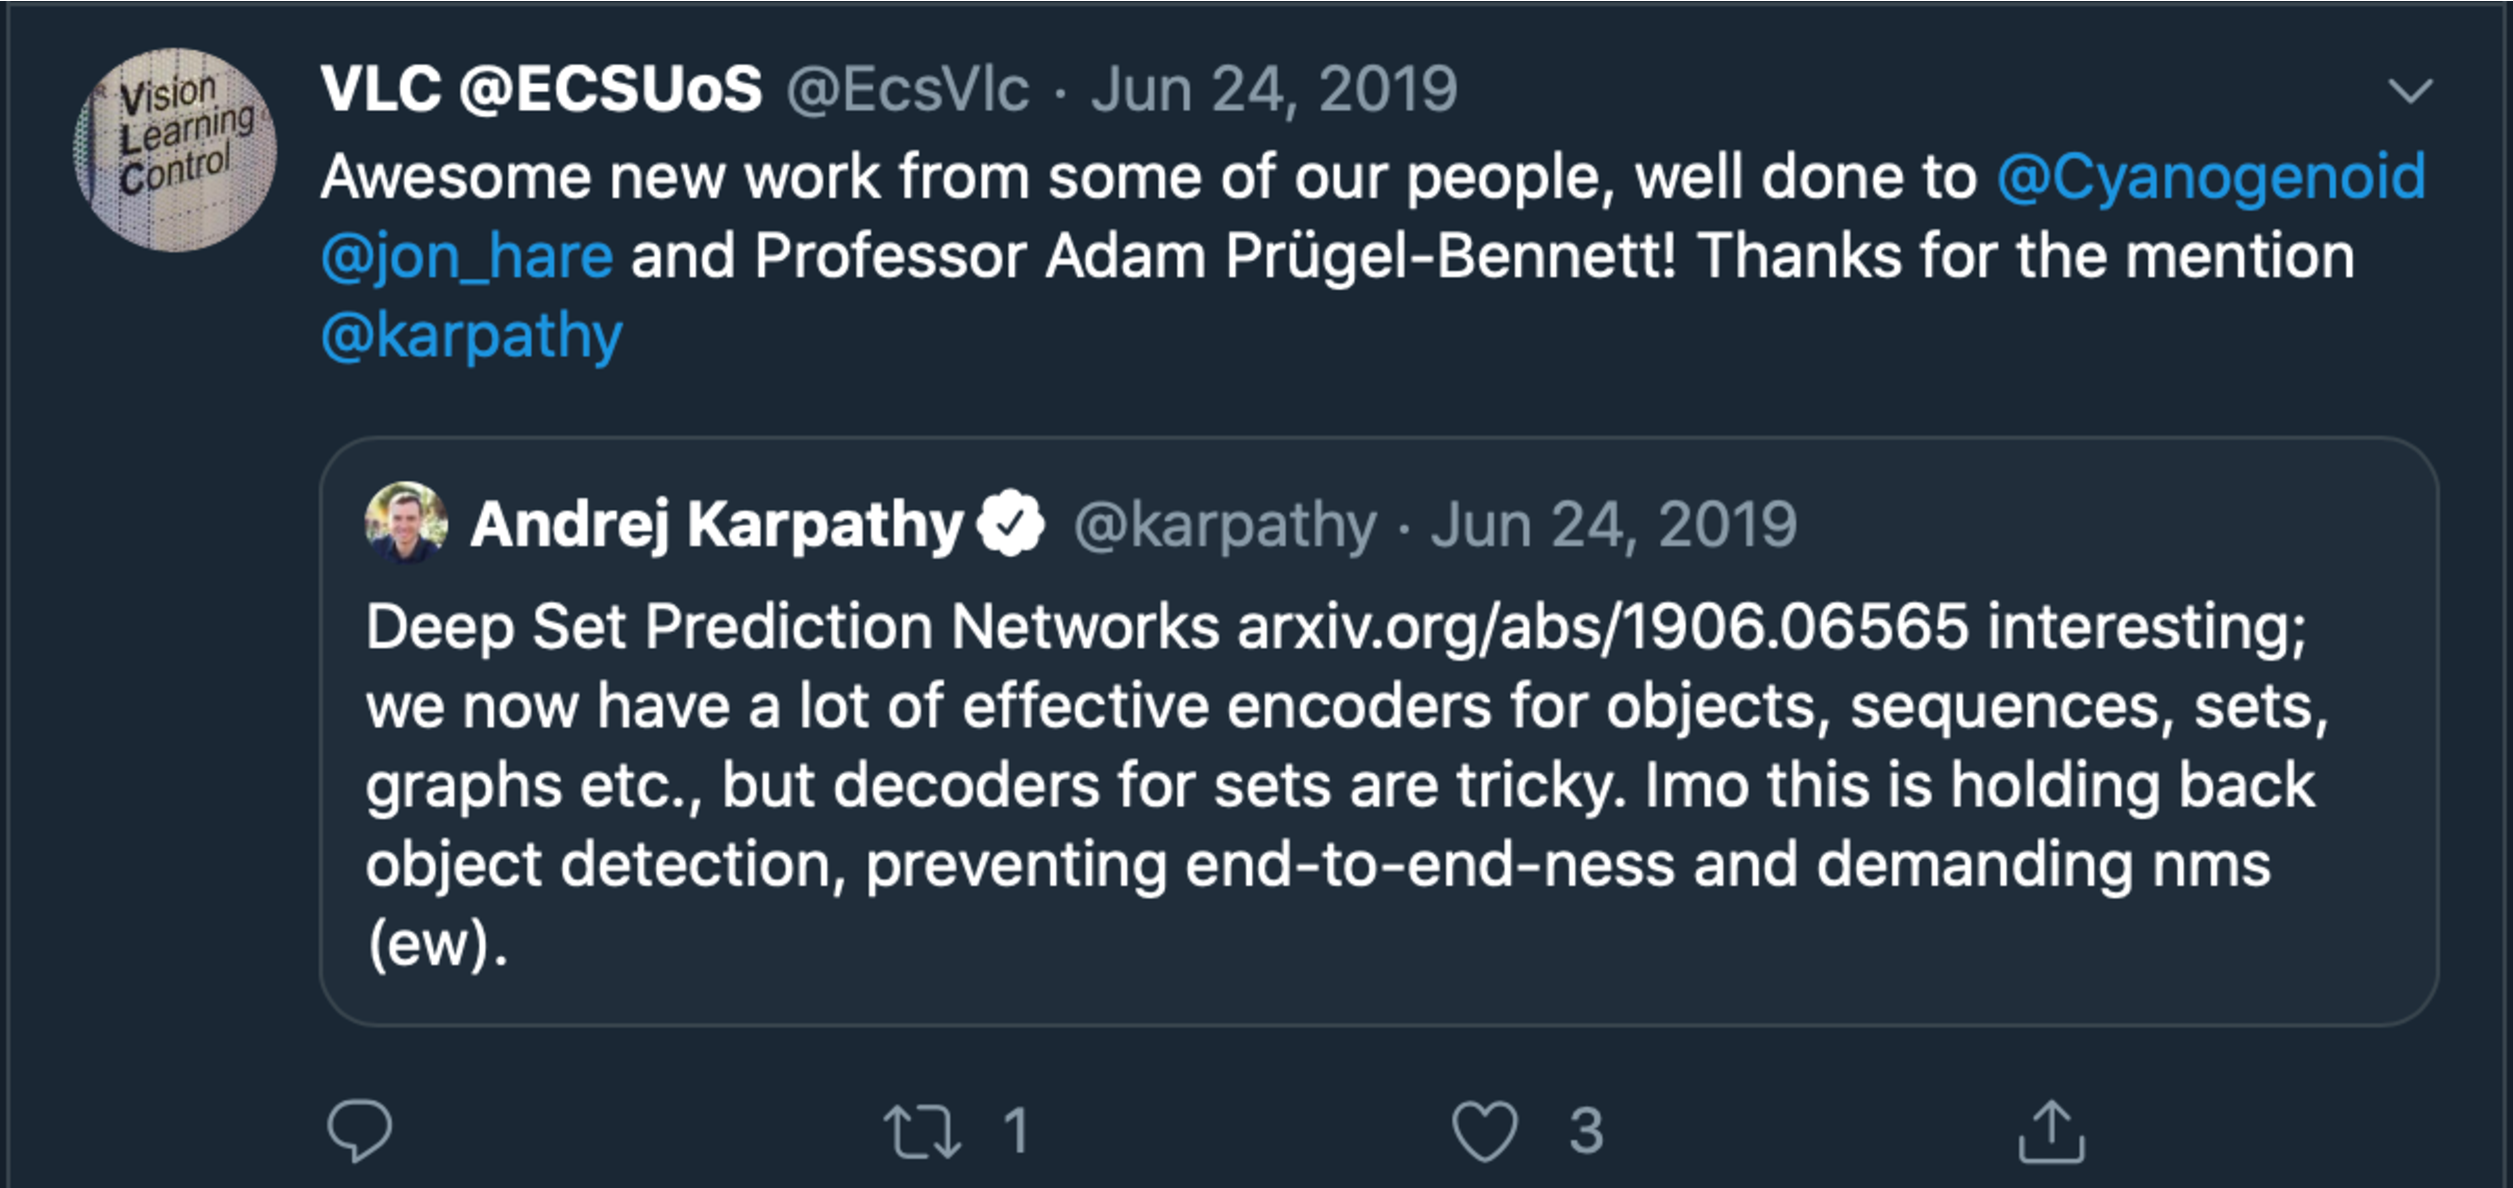
\includegraphics[width=10pc]{andrej}
  \end{flushright}
}
\end{frame}

\begin{frame}
  \frametitle{Topics}
  \begin{itemize}
    \item A quick look at an MLP again
    \item The chain rule (again)
    \item Uninititive gradient effects
    \item A closer look at basic stochastic gradient descent algorithms
  \end{itemize}
\end{frame}

\begin{frame}[fragile]\frametitle{The unbiased Multilayer Perceptron (again)...}
  \begin{center}
    \begin{tikzpicture}[shorten >=1pt,->,draw=black!50, node distance=\layersep]
        \tikzstyle{every pin edge}=[<-,shorten <=1pt]
        \tikzstyle{neuron}=[circle,fill=black!25,minimum size=17pt,inner sep=0pt]
        \tikzstyle{input neuron}=[neuron, fill=green!50];
        \tikzstyle{output neuron}=[neuron, fill=red!50];
        \tikzstyle{hidden neuron}=[neuron, fill=blue!50];
        \tikzstyle{annot} = [text width=4em, text centered]

        % Draw the input layer nodes
        \foreach \name / \y in {1,...,4}
        % This is the same as writing \foreach \name / \y in {1/1,2/2,3/3,4/4}
            \node[input neuron] (I-\name) at (0,-\y) {$x_\y$};

        % Draw the hidden layer nodes
        \foreach \name / \y in {1,...,5}
            \path[yshift=0.5cm]
                node[hidden neuron] (H-\name) at (1.5*\layersep,-\y cm) {$h_\y$};

        % Draw the output layer node
            \foreach \name / \y in {1,...,2}
            \path[yshift=0.5cm]
                node[output neuron, pin={[pin edge={->}]right:$\hat y_\y$}, right of=H-3] (O-\name) at (1.5*\layersep,-40-\y cm) {$o_\y$};
        %\node[output neuron,pin={[pin edge={->}]right:Output}, right of=H-3] (O) {o};

        % Connect every node in the input layer with every node in the
        % hidden layer.
        \path (I-1) edge node[anchor=south] {$w_{ji}^{(1)}$}(H-1);
       \foreach \source in {1,...,4}
            \foreach \dest in {1,...,5}
           % \draw [arrow] (I-\source) - (H-\dest);
                \path (I-\source) edge (H-\dest) ;

        % Connect every node in the hidden layer with the output layer
        \path (H-1) edge node[anchor=south] {$w_{kj}^{(2)}$}(O-1);
        \foreach \source in {1,...,5}
           \foreach \dest in {1,...,2}
            \path (H-\source) edge (O-\dest);

        % Annotate the layers
        \node[annot,above of=H-1, node distance=1cm] (hl) {Hidden layer};
        \node[annot,left of=hl] {Input layer};
        \node[annot,right of=hl] {Output layer};
    \end{tikzpicture}
  \end{center}
  Without loss of generality, we can write the above as:
  \begin{center}
    $\hat{\bm y} = g(f(\bm x; \bm W^{(1)}); \bm W^{(2)}) = g(\bm{W}^{(2)} f(\bm{W}^{(1)} \bm x))$\\
  \end{center}
  where $f$ and $g$ are activation functions.
\end{frame}

\begin{frame}
  \frametitle{Gradients of our simple unbiased MLP}

\begin{itemize}
  \item<+-> Let's assume MSE Loss
  \begin{align*}
    \ell_{MSE}(\bm{\hat y}, \bm y) & = \|\bm{\hat y} - \bm y\|_2^2
  \end{align*}
  \item<+-> What are the gradients?
    \begin{equation*}
      \nabla_{\bm W^{*}} \ell_{MSE}(g(\bm{W}^{(2)} f(\bm{W}^{(1)} \bm x)), \bm y)
    \end{equation*}
  \item<+-> Clearly we need to apply the chain rule (vector form) multiple times
  \item<+-> We could do this by hand
  \item<+-> (But we're not that crazy!)
\end{itemize}
\end{frame}

\begin{frame}
  \frametitle{Let's go back to a simpler expression}

\uncover<+->{
  \begin{align*}
    f(x,y,z) & = (x+y)z \\
             & \equiv qz \; \mathrm{where} \; q=(x+y)     
  \end{align*}}
\uncover<+->{
  Clearly the partial derivatives of the subexpressions are trivial:
  \begin{align*}
    \partial f / \partial z = q \;\;\;\;\;\;\; \partial f / \partial q = z \\
    \partial q / \partial x = 1 \;\;\;\;\;\;\; \partial q / \partial y = 1 \\
  \end{align*}}
\uncover<+->{
  and the chain rule tells us how to combine these:
  \begin{align*}
    \partial f / \partial x & = \partial f / \partial q \cdot \partial q / \partial x = z\\
    \partial f / \partial y & = \partial f / \partial q \cdot \partial q / \partial y = z\\
  \end{align*}}
\uncover<+->{
  so $\nabla_{[x,y,z]} f = [z, z, q]$
}

\end{frame}

\begin{frame}[t]
  \frametitle{A computational graph perspective}

  \begin{align*}
    f(x,y,z) & = (x+y)z
  \end{align*}

  \only<handout>{
    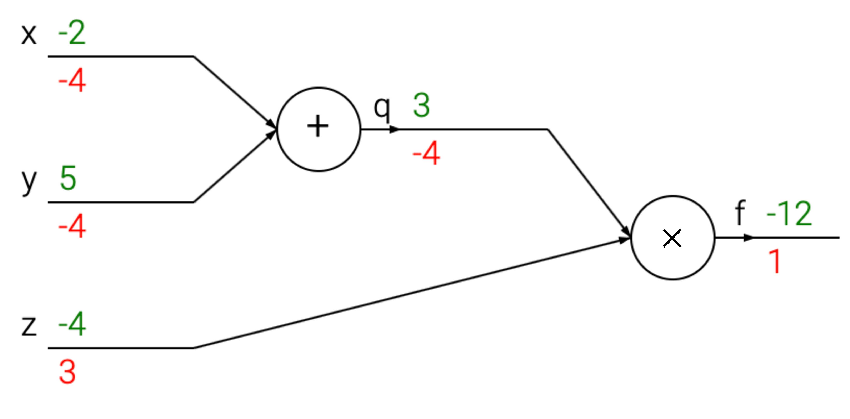
\includegraphics[width=\textwidth]{circuit.pdf}
  }
\end{frame}

\begin{frame}
  \frametitle{An intuition of the chain rule}

\begin{itemize}
  \item Notice how every operation in the computational graph given its inputs can immediately compute two things:
  \begin{enumerate}
    \item its output value
    \item the \emph{local} gradient of its inputs with respect to its output value
  \end{enumerate}
  \item The chain rule tells us literally that each operation should take its local gradients and multiply them by the gradient that \emph{flows} backwards into it
\end{itemize}
\end{frame}

\begin{frame}
  \frametitle{This is backpropagation}

\begin{itemize}
  \item<1-> The backprop algorithm is just the idea that you can perform the forward pass (computing and caching the local gradients as you go),
  \item<1-> and then perform a backward pass to compute the total gradient by applying the chain rule and re-utilising the cached local gradients
  \item<2-> Backprop is just another name for `Reverse Mode Automatic Differentiation'...
\end{itemize}
\end{frame}

\begin{frame}
  \frametitle{Unintuitive effects I: Multiplication}

\begin{itemize}
  \item<+-> Consider the multiplication operation $f(a,b) = a \times b$.
  \item<+-> The gradients are clearly $\partial f/\partial b = a$ and $\partial f/\partial a = b$.
  \begin{itemize}
    \item<+-> (in a computational graph these would be the local gradients w.r.t the inputs)
  \end{itemize}
  \item<+-> If $a$ is large and $b$ is tiny the gradient assigned to $b$ will be large, and the gradient to $a$ small.
  \item<+-> This has implications for e.g. linear classifiers ($\bm w^\top \bm x_i$) where you perform many multiplications
  \begin{itemize}
     \item<+-> the magnitude of the gradient is directly proportional to the magnitude of the data
     \item<+-> multiply $\bm x_i$  by 1000, and the gradients also increase by 1000
     \item<+-> if you don't lower the learning rate to compensate your model might not learn
     \item<+-> \textbf{Hence you need to always pay attention to data normalisation!}
   \end{itemize}
\end{itemize}
\end{frame}

\begin{frame}
  \frametitle{Unintuitive effects II: vanishing gradients of the sigmoid}
  \begin{itemize}
    \item<+-> It used to be popular to use sigmoids (or tanh) in the hidden layers...
    \item<+-> Gradient of $\sigma(x) = \sigma(x)(1-\sigma(x))$
    \item<+-> Thus as part of a larger network where this is the local gradient, if $x$ is large (+ve or -ve), then all gradients backwards from this point will be zero due to multiplication of the chain rule
    \begin{itemize}
      \item Why might $x$ be large?
    \end{itemize}
    \item<+-> Maximum gradient is achieved when $x=0$ \; ($\sigma(x)=0.5,\;dx=0.25$)
    \begin{itemize}
      \item<+-> This means that the maximum gradient that can flow out of a sigmoid will be a quarter of the input gradient
      \begin{itemize}
        \item<+-> What's the implication of this in a deep network with sigmoid activations?
      \end{itemize}
    \end{itemize}
  \end{itemize}
\end{frame}

\begin{frame}
  \frametitle{Unintuitive effects III: dying ReLUs}
  \begin{itemize}
    \item<+-> Modern networks tend to use ReLUs
    \item<+-> Gradient is $1$ for $x>0$ and $0$ otherwise
    \item<+-> Consider $\ReLU(\bm w^\top \bm x)$
    \begin{itemize}
      \item What happens if $\bm w$ is initialised badly?
      \item What happens if $\bm w$ receives an update that means that $\bm w^\top \bm x < 0 \; \forall \; \bm x$?
    \end{itemize}
    \item<+-> These are dead ReLUs - ones that never fire for all training data
    \begin{itemize}
      \item Sometimes you can find that you have a large fraction of these
      \item if you get them from the beginning, check weight initialisation and data normalisation
      \item if they're appearing during training, maybe $\lambda$ is too big?
    \end{itemize}
  \end{itemize}
\end{frame}

\begin{frame}
  \frametitle{Unintuitive effects IV: Exploding gradients in recurrent networks}
  \begin{itemize}
    \item<+-> Recurrent networks apply a function recursively for some number of timesteps
    \item<+-> Often this recursion involves a multiplication at each timestep, the gradients of which are all multiplied together because of the chain rule...
    \item<+-> Consider $z = a \prod_n^\infty b$
    \begin{itemize}
      \item<+-> $z \to 0\;if\;|b|<1$ 
      \item<+-> $z \to \infty\;if\;|b|>1$ 
    \end{itemize}
    \item<+-> Same thing happens in the backward pass of an RNN (although with matrices rather than scalars, so the reasoning applies to the largest eigenvalue)
  \end{itemize}
\end{frame}

\end{document}
